\documentclass{standalone}
\usepackage{tikz}
\usetikzlibrary{patterns, positioning}


\begin{document}
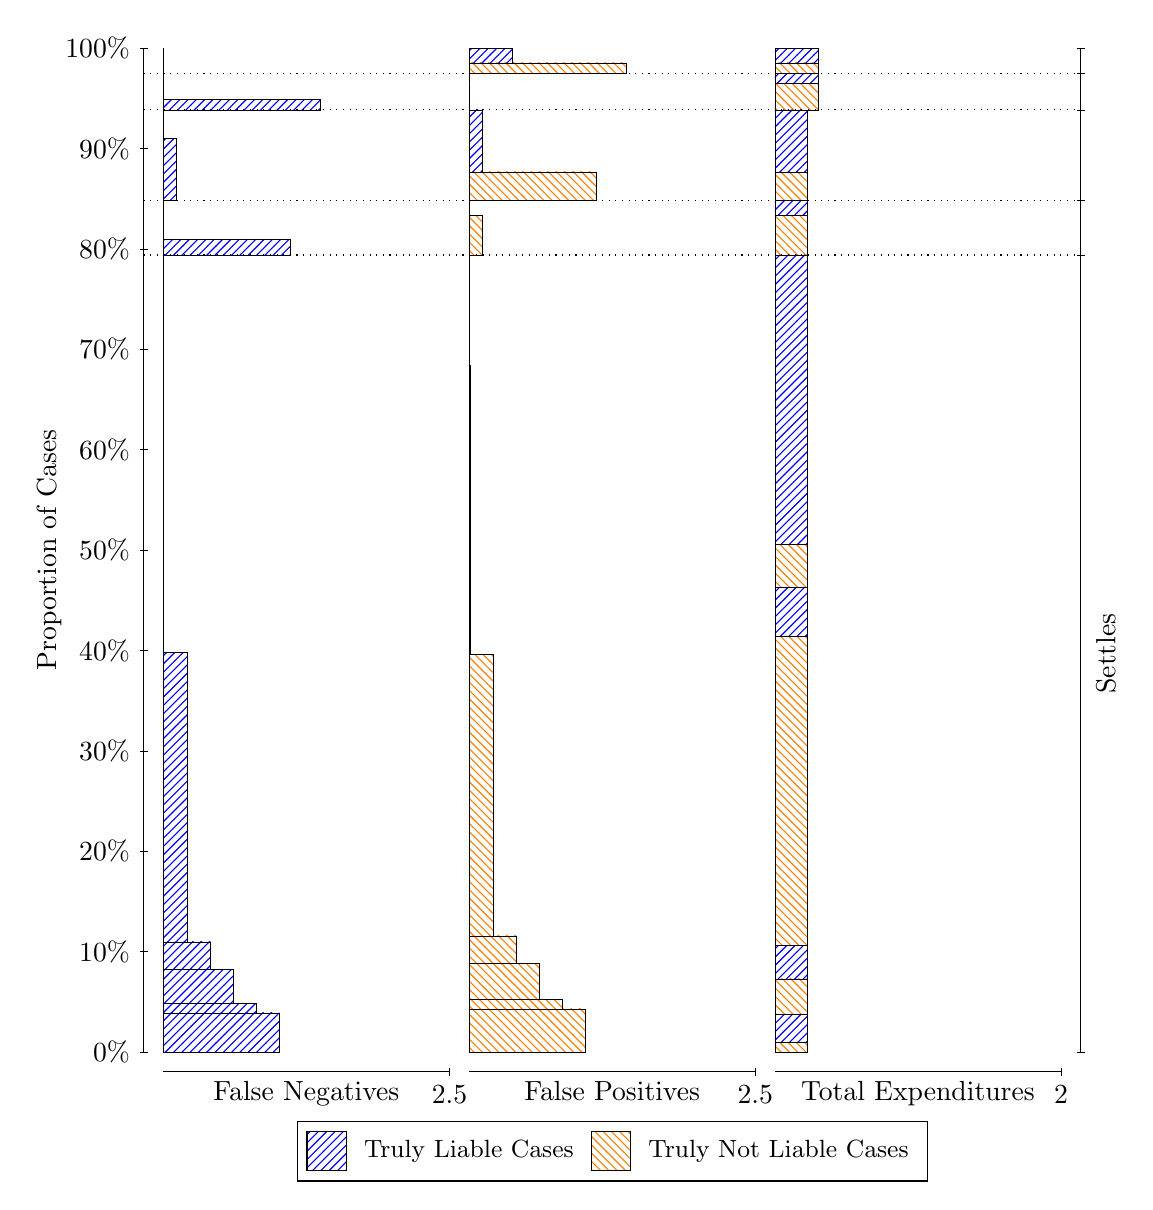
\begin{tikzpicture}
\draw[black, very thin] (1.5,1.75) -- (1.5,14.5);
\node[rotate=90, text=black, anchor=center] at (0.3, 8.125) {Proportion of Cases};
\draw[black, very thin] (1.45,1.75) -- (1.55,1.75);
\node[text=black, anchor=east] at (1.45, 1.75) {0\%};
\draw[black, very thin] (1.45,3.025) -- (1.55,3.025);
\node[text=black, anchor=east] at (1.45, 3.025) {10\%};
\draw[black, very thin] (1.45,4.3) -- (1.55,4.3);
\node[text=black, anchor=east] at (1.45, 4.3) {20\%};
\draw[black, very thin] (1.45,5.575) -- (1.55,5.575);
\node[text=black, anchor=east] at (1.45, 5.575) {30\%};
\draw[black, very thin] (1.45,6.85) -- (1.55,6.85);
\node[text=black, anchor=east] at (1.45, 6.85) {40\%};
\draw[black, very thin] (1.45,8.125) -- (1.55,8.125);
\node[text=black, anchor=east] at (1.45, 8.125) {50\%};
\draw[black, very thin] (1.45,9.4) -- (1.55,9.4);
\node[text=black, anchor=east] at (1.45, 9.4) {60\%};
\draw[black, very thin] (1.45,10.675) -- (1.55,10.675);
\node[text=black, anchor=east] at (1.45, 10.675) {70\%};
\draw[black, very thin] (1.45,11.95) -- (1.55,11.95);
\node[text=black, anchor=east] at (1.45, 11.95) {80\%};
\draw[black, very thin] (1.45,13.225) -- (1.55,13.225);
\node[text=black, anchor=east] at (1.45, 13.225) {90\%};
\draw[black, very thin] (1.45,14.5) -- (1.55,14.5);
\node[text=black, anchor=east] at (1.45, 14.5) {100\%};

\draw[black, very thin] (13.4,1.75) -- (13.4,14.5);
\draw[black, very thin] (13.35,1.75) -- (13.45,1.75);
\node[anchor=west] at (13.35, 1.75) {};
\draw[black, very thin] (13.35,11.872) -- (13.45,11.872);
\node[anchor=west] at (13.35, 11.872) {};
\draw[black, very thin] (13.35,12.567) -- (13.45,12.567);
\node[anchor=west] at (13.35, 12.567) {};
\draw[black, very thin] (13.35,13.714) -- (13.45,13.714);
\node[anchor=west] at (13.35, 13.714) {};
\draw[black, very thin] (13.35,14.181) -- (13.45,14.181);
\node[anchor=west] at (13.35, 14.181) {};
\draw[black, very thin] (13.35,14.5) -- (13.45,14.5);
\node[anchor=west] at (13.35, 14.5) {};

\draw[black, very thin, pattern color=blue, pattern=north east lines] (1.75,1.75) rectangle (3.2215,2.2478);
\draw[black, very thin, pattern color=blue, pattern=north east lines] (1.75,2.2478) rectangle (2.9308,2.371);
\draw[black, very thin, pattern color=blue, pattern=north east lines] (1.75,2.371) rectangle (2.6402,2.7971);
\draw[black, very thin, pattern color=blue, pattern=north east lines] (1.75,2.7971) rectangle (2.3495,3.1486);
\draw[black, very thin, pattern color=blue, pattern=north east lines] (1.75,3.1486) rectangle (2.0588,6.8242);
\draw[black, very thin, pattern color=orange, pattern=north west lines] (1.75,6.8242) rectangle (1.75,11.872);
\draw[black, very thin, pattern color=blue, pattern=north east lines] (1.75,11.872) rectangle (3.3668,12.066);
\draw[black, very thin, pattern color=orange, pattern=north west lines] (1.75,12.066) rectangle (1.75,12.567);
\draw[black, very thin, pattern color=blue, pattern=north east lines] (1.75,12.567) rectangle (1.9135,13.356);
\draw[black, very thin, pattern color=orange, pattern=north west lines] (1.75,13.356) rectangle (1.75,13.714);
\draw[black, very thin, pattern color=blue, pattern=north east lines] (1.75,13.714) rectangle (3.7483,13.843);
\draw[black, very thin, pattern color=orange, pattern=north west lines] (1.75,13.843) rectangle (1.75,14.181);
\draw[black, very thin, pattern color=orange, pattern=north west lines] (1.75,14.181) rectangle (1.75,14.31);
\draw[black, very thin, pattern color=blue, pattern=north east lines] (1.75,14.31) rectangle (1.75,14.5);
\draw[black, very thin, pattern color=orange, pattern=north west lines] (5.6333,1.75) rectangle (7.1048,2.2962);
\draw[black, very thin, pattern color=orange, pattern=north west lines] (5.6333,2.2962) rectangle (6.8142,2.4194);
\draw[black, very thin, pattern color=orange, pattern=north west lines] (5.6333,2.4194) rectangle (6.5235,2.8719);
\draw[black, very thin, pattern color=orange, pattern=north west lines] (5.6333,2.8719) rectangle (6.2328,3.2233);
\draw[black, very thin, pattern color=orange, pattern=north west lines] (5.6333,3.2233) rectangle (5.9422,6.798);
\draw[black, very thin, pattern color=blue, pattern=north east lines] (5.6333,6.798) rectangle (5.6515,10.474);
\draw[black, very thin, pattern color=blue, pattern=north east lines] (5.6333,10.474) rectangle (5.6333,11.872);
\draw[black, very thin, pattern color=orange, pattern=north west lines] (5.6333,11.872) rectangle (5.7968,12.374);
\draw[black, very thin, pattern color=blue, pattern=north east lines] (5.6333,12.374) rectangle (5.6333,12.567);
\draw[black, very thin, pattern color=orange, pattern=north west lines] (5.6333,12.567) rectangle (7.2502,12.926);
\draw[black, very thin, pattern color=blue, pattern=north east lines] (5.6333,12.926) rectangle (5.7968,13.714);
\draw[black, very thin, pattern color=orange, pattern=north west lines] (5.6333,13.714) rectangle (5.6333,14.052);
\draw[black, very thin, pattern color=blue, pattern=north east lines] (5.6333,14.052) rectangle (5.6333,14.181);
\draw[black, very thin, pattern color=orange, pattern=north west lines] (5.6333,14.181) rectangle (7.6317,14.31);
\draw[black, very thin, pattern color=blue, pattern=north east lines] (5.6333,14.31) rectangle (6.1783,14.5);
\draw[black, very thin, pattern color=orange, pattern=north west lines] (9.5167,1.75) rectangle (9.9254,1.8732);
\draw[black, very thin, pattern color=blue, pattern=north east lines] (9.5167,1.8732) rectangle (9.9254,2.2247);
\draw[black, very thin, pattern color=orange, pattern=north west lines] (9.5167,2.2247) rectangle (9.9254,2.6771);
\draw[black, very thin, pattern color=blue, pattern=north east lines] (9.5167,2.6771) rectangle (9.9254,3.1033);
\draw[black, very thin, pattern color=orange, pattern=north west lines] (9.5167,3.1033) rectangle (9.9254,7.0294);
\draw[black, very thin, pattern color=blue, pattern=north east lines] (9.5167,7.0294) rectangle (9.9254,7.6504);
\draw[black, very thin, pattern color=orange, pattern=north west lines] (9.5167,7.6504) rectangle (9.9254,8.1965);
\draw[black, very thin, pattern color=blue, pattern=north east lines] (9.5167,8.1965) rectangle (9.9254,11.872);
\draw[black, very thin, pattern color=orange, pattern=north west lines] (9.5167,11.872) rectangle (9.9254,12.374);
\draw[black, very thin, pattern color=blue, pattern=north east lines] (9.5167,12.374) rectangle (9.9254,12.567);
\draw[black, very thin, pattern color=orange, pattern=north west lines] (9.5167,12.567) rectangle (9.9254,12.926);
\draw[black, very thin, pattern color=blue, pattern=north east lines] (9.5167,12.926) rectangle (9.9254,13.714);
\draw[black, very thin, pattern color=orange, pattern=north west lines] (9.5167,13.714) rectangle (10.062,14.052);
\draw[black, very thin, pattern color=blue, pattern=north east lines] (9.5167,14.052) rectangle (10.062,14.181);
\draw[black, very thin, pattern color=orange, pattern=north west lines] (9.5167,14.181) rectangle (10.062,14.31);
\draw[black, very thin, pattern color=blue, pattern=north east lines] (9.5167,14.31) rectangle (10.062,14.5);
\draw[black, dotted] (1.5,11.872) -- (13.4,11.872);
\draw[black, dotted] (1.5,12.567) -- (13.4,12.567);
\draw[black, dotted] (1.5,13.714) -- (13.4,13.714);
\draw[black, dotted] (1.5,14.181) -- (13.4,14.181);
\draw[black, very thin] (1.75,1.5) -- (5.3833,1.5);
\node[text=black, anchor=north] at (3.5667, 1.5) {False Negatives};
\draw[black, very thin] (5.3833,1.45) -- (5.3833,1.55);
\node[text=black, anchor=north] at (5.3833, 1.45) {2.5};

\draw[black, very thin] (5.6333,1.5) -- (9.2667,1.5);
\node[text=black, anchor=north] at (7.45, 1.5) {False Positives};
\draw[black, very thin] (9.2667,1.45) -- (9.2667,1.55);
\node[text=black, anchor=north] at (9.2667, 1.45) {2.5};

\draw[black, very thin] (9.5167,1.5) -- (13.15,1.5);
\node[text=black, anchor=north] at (11.333, 1.5) {Total Expenditures};
\draw[black, very thin] (13.15,1.45) -- (13.15,1.55);
\node[text=black, anchor=north] at (13.15, 1.45) {2};

\node[text=black, centered, rotate=90] at (13.72, 6.8111) {Settles};





\draw (7.449999999999999,1.5) node[draw=none] (baseCoordinate) {};
\begin{scope}[align=center]
        \matrix[scale=0.5, draw=black, below=0.5cm of baseCoordinate, nodes={draw}, column sep=0.1cm]{
            \node[rectangle, draw, minimum width=0.5cm, minimum height=0.5cm, pattern color=blue, pattern=north east lines] {}; &
            \node[draw=none, font=\small, text=black] (B) {Truly Liable Cases}; &
            \node[rectangle, draw, minimum width=0.5cm, minimum height=0.5cm, pattern color=orange, pattern=north west lines] {}; &
            \node[draw=none, font=\small, text=black] (B) {Truly Not Liable Cases}; \\
            };
\end{scope}

\end{tikzpicture}
\end{document}